\documentclass[10pt]{beamer}

\usepackage[utf8x]{inputenc}
\usepackage{listings}
\usepackage{tikz}
\usepackage{xspace}
\usepackage{ulem}

\usepackage{amsmath,amsfonts,amssymb}
\newcommand{\E}{\ensuremath{\textnormal{E}}}
\newcommand{\Var}{\ensuremath{\textnormal{Var}}}
\DeclareMathOperator{\erf}{erf}


\definecolor{sagepurple}{HTML}{7474DB}
\definecolor{oxygenorange}{HTML}{F26F21}
\definecolor{oxygengray}{HTML}{686868}
\definecolor{oxygenlightgray}{HTML}{EEEEEE}
\definecolor{oxygenblue}{HTML}{236EAF}

\mode<presentation>
{
  \usetheme{Rochester}
  \usefonttheme{serif}
  \setbeamercovered{transparent}
  \setbeamercolor{structure}{fg=oxygenblue}
  \setbeamercolor{block title}{bg=oxygenblue,fg=white}
  \setbeamercolor{block body}{bg=oxygenlightgray,fg=black}
}

\AtBeginSection[]{
   \begin{frame}
       \frametitle{Outline}
       \tableofcontents[currentsection]
   \end{frame}
}

\lstdefinelanguage{Sage}[]{Python}{morekeywords={True,False,sage,cdef,cpdef,ctypedef,self},sensitive=true}

\lstset{frame=none,
          showtabs=False,
          showspaces=False,
          showstringspaces=False,
          commentstyle={\color{oxygenorange}\bfseries},
          keywordstyle={\color{oxygenblue}\bfseries},
          stringstyle ={\color{oxygengray}},
          language = Sage,
          basicstyle=\scriptsize\tt
          }

\newcommand{\field}[1]{\mathbb{#1}}
\newcommand{\F}{\field{F}}
\newcommand{\PolyBoRi}{\textsc{PolyBoRi}\xspace}
\newcommand{\Magma}{\textsc{Magma}\xspace}
\newcommand{\Singular}{\textsc{Singular}\xspace}
\renewcommand{\emph}[1]{\textbf{\color{oxygenblue}#1}}
\newcommand{\getinvolved}[1]{\begin{block}{Get Involved!}#1\end{block}}

\title{Sage for Cryptographers}
\author{Martin R.\ Albrecht (martinralbrecht+summerschool@googlemail.com)}
\institute{POLSYS Team, UPMC, Paris, France}
\titlegraphic{
\includegraphics[width=0.2\textwidth]{sage-logo-new.png}}
\date{ECrypt II PhD Summer School}

\begin{document}

\begin{frame}
\titlepage
\end{frame}

\begin{frame}{Outline}
\tableofcontents
\end{frame}

\section{Introduction}

\begin{frame}[fragile]
\frametitle{A Few Examples}
\begin{lstlisting}
sage: 1+1
2

sage: A = random_matrix(GF(2),10000,10000)
sage: A.echelon_form()
10000 x 10000 dense matrix over Finite Field of size 2

sage: A = random_matrix(ZZ, 100, 100, x=-2^16,y=2^16)
sage: A.LLL()
100 x 100 dense matrix over Integer Ring

sage: A.hermite_form()
100 x 100 dense matrix over Integer Ring

sage: sr = mq.SR(1,2,2,4,gf2=True,polybori=True) # small AES
sage: F,s = sr.polynomial_system()
sage: F.groebner_basis()
Polynomial Sequence with 72 Polynomials in 72 Variables
\end{lstlisting}
\end{frame}

\begin{frame}
\frametitle{Blurb}

\begin{columns}

\column{0.15\textwidth}

\begin{center}
 
\includegraphics[height=0.95\textwidth]{./sage-logo.png}
\end{center}

\column{0.8\textwidth}
\begin{block}{Sage open-source mathematical software system}
``Creating a viable free open source alternative to Magma, Maple, Mathematica and Matlab.''
\end{block}
\end{columns}

\vspace{1em}

Sage is a free open-source mathematics software system licensed under the GPL. It combines the power of many existing open-source packages into a common Python-based interface.

\vspace{1em}

\begin{tabular}{ll}
First release 2005 & Latest version 5.0 released 2012-05-14\\
$>$ 300 Releases  & Shell, webbrowser (GUI), library\\
$>$ 180 Developers  & $\sim 100$ Components\\
$>$ 100 papers cite Sage & $> 2100$ subscribers [sage-support]\\
$>$ 100,000 web visitors/month&  $> 6,500$ downloads/month\\
\end{tabular}
\end{frame}

\begin{frame}
\frametitle{How to use it}
Sage can be used via the command line, as a webapp hosted on your local computer and via the Internet, or embedded on any website.

\begin{center}
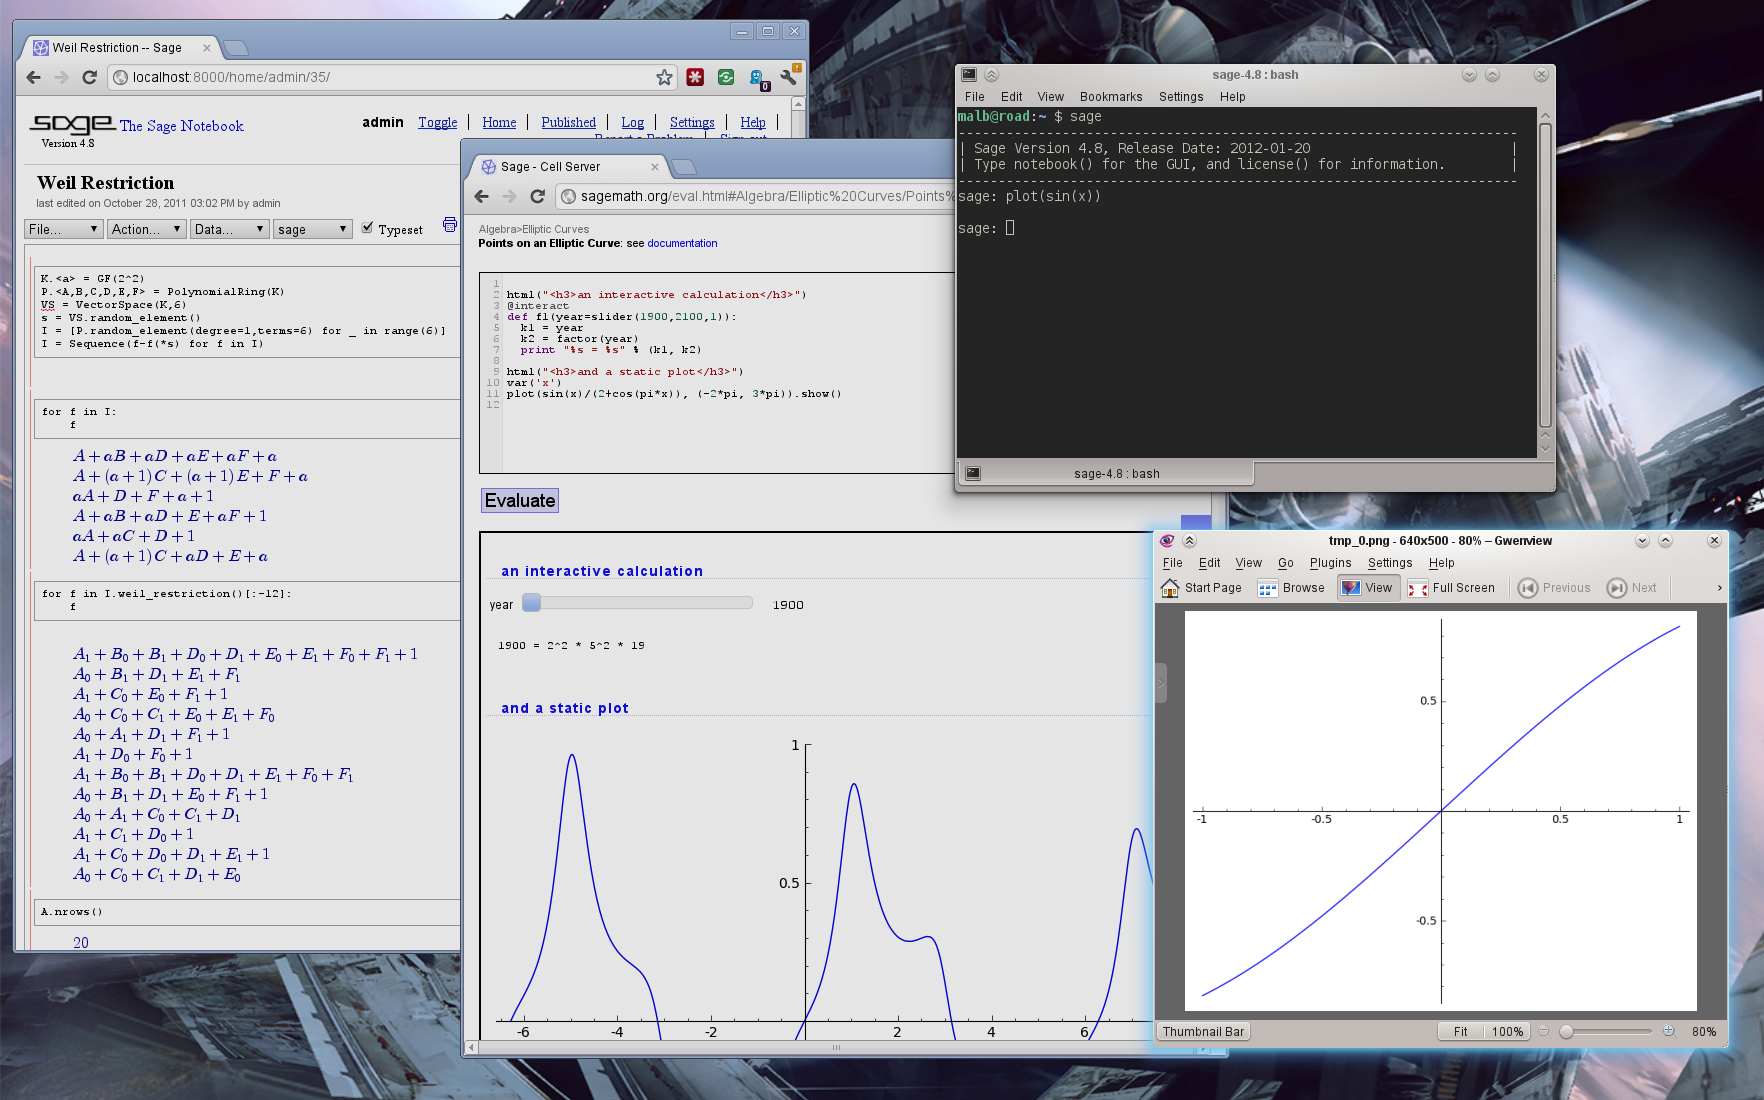
\includegraphics[width=0.8\textwidth]{sage-desktop.png}
\end{center}

\end{frame}


\begin{frame}
\frametitle{``How do I do \dots in Sage?''}
\framesubtitle{\hfill \dots It's easy: implement it and send us a patch.}

Sage is a largely volunteer-driven effort, this means that
\begin{itemize}
 \item developers work on whatever suits their needs best;
 \item the quality of code in Sage varies:
 \begin{itemize}
   \item is a generic or a specialised, optimised implementation used,
   \item how much attention is paid to details,
   \item is your application an untested ``corner case'',
   \item how extensive are the tests, the documentation, or
   \item is the version of a particular package up to date.
 \end{itemize}
 \item you cannot expect people to fix your favourite bug quickly (although we do try!),
 \item you can get involved and make Sage better for your needs!
\end{itemize}


\begin{block}{Get involved}
I will highlight relevant issues to encourage you to get involved.
\end{block}
\end{frame}

\section{Highlevel Features}

\begin{frame}[fragile]
\frametitle{Python \& Cython}
\begin{center}
 
\includegraphics[width=0.4\textwidth]{python-and-cython.png}
\end{center}

Sage does \emph{not} come with yet-another ad-hoc mathematical programming language, it uses
\emph{Python} instead.

\begin{itemize}
\item one of the most widely used programming languages (Google, IML, YouTube, NASA),
\item easy for you to define your own data types and methods on it (bitstreams, ciphers, rings, whatever),
\item very clean language that results in easy to read code,
\item a \emph{huge number of libraries}: statistics, networking, databases,
bioinformatic, physics, video games, 3d graphics, numerical computation (scipy),
and serious ``pure'' mathematics (via Sage)
\item easy to use existing C/C++ libraries from Python (via \emph{Cython})
\end{itemize}
\end{frame}



\begin{frame}[fragile]
\frametitle{Python Example: Databases}

\begin{lstlisting}
sage: import sqlalchemy as S
sage: db = S.create_engine('sqlite:///tutorial.db')
sage: users = S.Table('users', S.MetaData(db),
              S.Column('user_id', S.Integer, primary_key=True),
              S.Column('name', S.String(40r)),
              S.Column('modulus', S.String)).create()

sage: i = users.insert()
sage: M = random_prime(2^512)*random_prime(2^512)
sage: i.execute(name='Mary',modulus=str(M))

sage: s = users.select(whereclause="name='Mary'")
sage: row = s.execute().fetchone()
sage: ZZ(row[users.c.modulus])
56974631402866323...250077669
\end{lstlisting}

\end{frame}

\begin{frame}[fragile]
\frametitle{Python Example: Networking}
\begin{small}
\emph{Scapy} is a powerful interactive packet manipulation program written in Python. It is able to forge or decode packets of a wide number of protocols, send them on the wire, capture them, match requests and replies, and much more. It can easily handle most classical tasks like scanning, tracerouting, probing, unit tests, attacks or network discovery.
\end{small}

\begin{lstlisting}
from scapy.all import *

class Test(Packet):
    name = "Test packet"
    fields_desc = [ ShortField("test1", 1),
                    ShortField("test2", 2) ]

print Ether()/IP()/Test(test1=x,test2=y)

p=sr1(IP(dst="127.0.0.1")/ICMP())
if p:
    p.show()
\end{lstlisting}
\end{frame}

\begin{frame}[fragile]
\frametitle{Cython: Your Own Code}
\begin{lstlisting}
sage: cython("""
def foo(unsigned long a, unsigned long b):
  cdef int i
  for i in range(64):
    a ^= a*(b<<i)
  return a
""")
sage: foo(a,b)
\end{lstlisting}

\vspace{1em}

This generates C code like this:

\begin{lstlisting}[language=c]
for (__pyx_t_1 = 0; __pyx_t_1 < 64; __pyx_t_1+=1) {
    __pyx_v_i = __pyx_t_1;
    __pyx_v_a = (__pyx_v_a ^ _pyx_v_a * (__pyx_v_b << __pyx_v_i));
}
\end{lstlisting}
\end{frame}

\begin{frame}[fragile,allowframebreaks]
\frametitle{Cython: External Code}
\begin{lstlisting}
#cargs -std=c99 -ggdb
cdef extern from "katan.c":
    ctypedef unsigned long uint64_t
    void katan32_encrypt(uint64_t *p, uint64_t *c, uint64_t *k, int nr)
    void katan32_keyschedule(uint64_t *k, uint64_t *key, int br)
    uint64_t ONES

def k32_encrypt(plain, key):
    cdef int i
    cdef uint64_t _plain[32], _cipher[32], kk[2*254], _key[80]

    for i in range(80):
        _key[i] = ONES if key[i] else 0
    for i in range(32):
        _plain[i] = ONES if plain[i] else 0

    katan32_keyschedule(kk, _key, 254)
    katan32_encrypt(_plain, _cipher, _key, 254)

    return [int(_cipher[i]%2) for i in range(32)]

sage: attach "sage-katan.spyx"
sage: k32_encrypt(random_vector(GF(2),32),random_vector(GF(2),80))
[1, 0, 0, 1, 0, 1, 0, 0, 0, 1, ... 0, 1, 0, 0]
\end{lstlisting}

\framebreak


\begin{lstlisting}
sage: rv = lambda : random_vector(GF(2),32)
sage: E = lambda : k32_encrypt(rv(),rv())

sage: l = [E() for _ in range(1024)]
sage: l = [sum(e) for e in l]
sage: r.summary(l) # We are using R!
Min. 1st Qu.  Median    Mean 3rd Qu.    Max.
8.00   14.00   16.00   16.03   18.00   27.00

sage: c = E()
sage: K = GF(next_prime(2^32))
sage: g = K(sum(2^i*c[i] for i in range(32))); g
2859908881
sage: g.multiplicative_order() # We are using Pari/GP
858993462

sage: A = matrix(GF(2),32,32,[E() for _ in range(32)])
sage: A.rank() # We are using M4RI
30
\end{lstlisting}


\end{frame}


\begin{frame}[fragile]
\frametitle{Symmetric Multiprocessing}

\sout{Embarrassingly} proudly parallel computations on multicore machines are easy in Sage:

\begin{lstlisting}
sage: @parallel(2)
....: def f(n):
....:     return factor(n)
....:

sage: %time _ = [f(2^217-1), f(2^217-1)]
CPU times: user 1.07 s, sys: 0.02 s, total: 1.09 s
Wall time: 1.10 s

sage: %time _ = list( f([2^217-1, 2^217-1]) )
CPU times: user 0.00 s, sys: 0.02 s, total: 0.02 s
Wall time: 0.62 s

sage: 1.08/0.62
1.74193548387097
\end{lstlisting}
\end{frame}

\section{Mathematics}

\begin{frame}[fragile,allowframebreaks]
\frametitle{Dense Linear Algebra}

\begin{center}
\footnotesize
\begin{tabular}{|l|l|l|}
\hline
 \textbf{Base Ring}  & \textbf{Implementation} & \textbf{Comments}\\
\hline
 $\F_{2^e}$ $1 \leq e\leq 10$ & {\tt M4RI}, {\tt M4RIE} & Very good\\
 $\F_p$, $p=3,5,7,\dots$      & {\tt LinBox}            & Decent\\
 $\F_p$, $p<2^{22}$ prime     & {\tt LinBox}            & Very good\\
 $\F_{p^k}$                   &  Generic                & Very poor\\
\hline
 $\field{Q},\field{Z}$        & {\tt LinBox}, {\tt Pari}, {\tt IML}, {\tt NTL}, custom & Decent, fastest HNF\\
 $\field{R},\field{C}$ 53-bit & {\tt NumPy} + {\tt ATLAS}  & Very good\\
 $\field{Q}(\zeta_n)$         & Custom                  & Very good \\
\hline
 $\field{K}[x]$ & Generic & Very poor\\
 $\field{K}[x_0,\dots,x_{n-1}]$ & {\tt Singular}, generic & Mixed\\
\hline
\end{tabular}
\end{center}

\framebreak

\begin{lstlisting}
sage: for p in (2,3,4,5,7,8,9,11):
....:     K = GF(p,'a')
....:     A = random_matrix(K,2000,2000)
....:     B = random_matrix(K,2000,2000)
....:     t = cputime()
....:     C = A*B
....:     print "%32s %7.3f"%(K,cputime(t))
....:
Finite Field of size 2          0.008 # M4RI
Finite Field of size 3          0.972 # LinBox
Finite Field in a of size 2^2   0.048 # M4RIE
Finite Field of size 5          0.996 # LinBox
Finite Field of size 7          0.968 # LinBox
Finite Field in a of size 2^3   0.072 # M4RIE
Finite Field in a of size 3^2 695.863 # generic
Finite Field of size 11         1.020 # LinBox
\end{lstlisting}

\getinvolved{We are currently working on improving $\F_{p^k}$.
{\tt FLINT} 2.3 improves $\F_p$ for $p<2^{64}$.}

\end{frame}

\begin{frame}[fragile]
\frametitle{Sparse Linear Algebra}

Sage allows to construct and to compute with sparse matrices using the {\tt sparse=True} keyword.

\begin{lstlisting}
sage: A = random_matrix(GF(32003),2000,2000,density=~200,sparse=True)
sage: %time copy(A).rank() # LinBox
CPU times: user 3.26 s, sys: 0.05 s, total: 3.31 s
Wall time: 3.33 s
2000
sage: %time copy(A).echelonize() # custom code
CPU times: user 9.51 s, sys: 0.02 s, total: 9.52 s
Wall time: 9.56 s
sage: v = random_vector(GF(32003),2000)
sage: %time _ = copy(A).solve_right(v) # LinBox + custom code
CPU times: user 3.74 s, sys: 0.00 s, total: 3.74 s
Wall time: 3.76 s
\end{lstlisting}

\getinvolved{\texttt{LinBox}'s claim to fame is good support for \emph{black box} algorithms for sparse and structured matrices. Help us to expose more of this functionality.}
\end{frame}

\begin{frame}[fragile, allowframebreaks]
\frametitle{Lattices}
Sage includes both \texttt{NTL} and \texttt{fpLLL}:

\begin{lstlisting}
sage: from sage.libs.fplll.fplll import gen_intrel  # Knapsack-style
sage: A = gen_intrel(50,50); A
50 x 51 dense matrix over Integer Ring ...
sage: min(v.norm().n() for v in A.rows())
2.17859318110950e13

sage: L = A.LLL() # using fpLLL, NTL optional
sage: L[0].norm().n()
5.47722557505166

sage: L = A.BKZ() # using NTL
sage: L[0].norm().n()
3.60555127546399
\end{lstlisting}

\framebreak

Coppersmith's method for finding small roots is available:

\begin{lstlisting}
sage: N = 10001
sage: K = Zmod(10001)
sage: P.<x> = PolynomialRing(K)
sage: f = x^3 + 10*x^2 + 5000*x - 222
sage: f.small_roots()
[4]
\end{lstlisting}

\getinvolved{
\begin{itemize}
 \item our version of {\tt fpLLL} is very old,
 \item {\tt fpLLL} 4.0 has an implementation of BKZ, and
 \item there is no \texttt{Lattice} class for e.g. \texttt{L.shortest\_vector(gap=x)},
\end{itemize}
 but improving this is a Google Summer of Code 2012 project.}


\end{frame}

\begin{frame}[fragile]
\frametitle{Combinatorics}
\begin{lstlisting}
sage: IV3 = IntegerVectors(3,10)
sage: IV3.random_element()
[0, 0, 1, 0, 0, 2, 0, 0, 0, 0]

sage: C = Combinations(range(100),10); C
Combinations of [0, 1, 2, 3, 4, ..., 98, 99] of length 10
sage: C.cardinality()
17310309456440
\end{lstlisting}

Sage also has a very active (algebraic) combinatorics group.

\begin{block}{}
You can tell by the lack of examples how badly I suck at combinatorics \dots there's lots and lots in Sage.
\end{block}


\end{frame}

\begin{frame}[fragile]
\frametitle{Symbolics}
Sage uses {\tt Pynac} ({\tt GiNaC} fork) and {\tt Maxima} for most of its symbolic manipulation. {\tt SymPy} is included in Sage as well.

\begin{lstlisting}
sage: q = var('q')
sage: expr = (1-1/q)/(q-1)
sage: f = expr.function(q); f
q |--> -(1/q - 1)/(q - 1)
sage: f(10)
1/10
sage: f(q^2)
-(1/q^2 - 1)/(q^2 - 1)
sage: f(0.1)
10.0000000000000
sage: g = P.random_element(); g
4*x^2 + 3/4*x
sage: f(g)
-4*(4/((16*x + 3)*x) - 1)/((16*x + 3)*x - 4)

sage: expr.simplify_full()
1/q
sage: expr.integrate(q)
log(q)
\end{lstlisting}
\end{frame}

\begin{frame}[fragile,allowframebreaks]
\frametitle{Numerical Root Finding and Approximation}

Assume, we want have two counters: one for a correct key guess and one for an incorrect guess. Assume further that these counters are distributed according $\mathcal{N}(\E_c,\Var_c)$ and $\mathcal{N}(\E_w,\Var_w)$. We want to know how many samples we need to distinguish these two distributions for 50\% of the keys. That is, we want to solve

$$1-e^n < \frac{1}{2}\left(1+\erf\left(\frac{\E_c(n) -\E_w(n)}{\sqrt{2 \Var_w(n)/m}} \right)\right) \mbox{ for } m.$$

\framebreak

First, we compute some data by numerically solving for $m$:

\begin{lstlisting}
sage: n,m = var('n,m')
...
sage: f = 1/2 * (1 + erf( (E_c(n,m) - E_w(n,m))/
                          (sqrt(2*Var_w(n,m))) ) - (1 - e^n)
sage: l = []
sage: for n in range(64,256+1,8):
...      f_n = f.subs(n=n).function(m)
...      m = ceil(f_n.find_root(32,2**40)
...      l.append( (n,m) )
\end{lstlisting}

\framebreak

Now, we approximate this data numerically under the assumption that $m = \mathrm{poly}(n)$

\begin{lstlisting}
sage: n,c,a,b = var('n,c,a,b')
sage: model = (a*n**c + b).function(n)
sage: s = find_fit(l, model, solution_dict=True)
sage: m = model.subs(s); m
n |--> 0.021639206984895312*n^1.5496891146692116 + 89.975123416726277
\end{lstlisting}

Hence, we have $m \approx 0.022 \cdot n^{1.55} + 90.$

\end{frame}


\begin{frame}[fragile,allowframebreaks]
\frametitle{Statistics}
Sage ships {\tt R} which is a very powerful package for doing statistics, Sage also uses {\tt SciPy} for stats related tasks.

\begin{lstlisting}
sage: O() # some oracle
sage: l = [O() for _ in range(10000)] # we sample it
sage: r.summary(l) # and ask R about it
  Min.  1st Qu.   Median     Mean  3rd Qu.     Max.
-154.000  -31.000    2.000    0.298   33.000  140.000
sage: import pylab # use pylab to compute a histogram
sage: a,b,_ = pylab.hist(l,100)
sage: line(zip(b,a)) # and Sage's code to plot it
\end{lstlisting}

\begin{columns}
\column{0.5\textwidth}
\centering
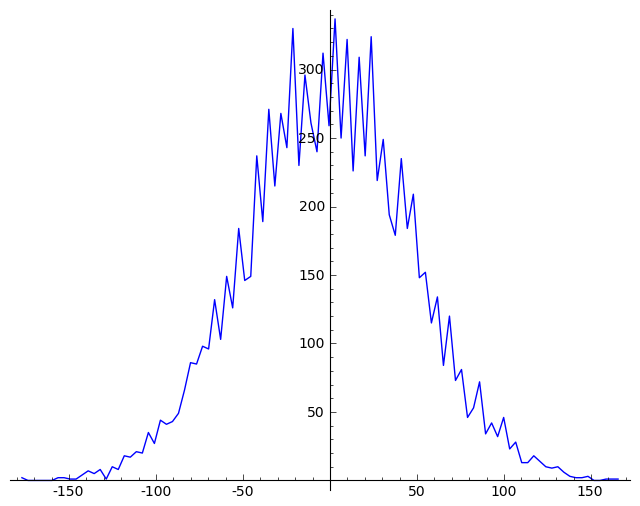
\includegraphics[width=0.7\textwidth]{gaussian.png}
\column{0.5\textwidth}
\getinvolved{Our interface to R could be greatly improved}
\end{columns}

\framebreak

Looks kinda Gaussian, doesn't it.

\begin{lstlisting}
sage: T = RealDistribution('gaussian',variance(l).sqrt())
sage: T.cum_distribution_function(5)
0.542044391014

sage: mu = mean(l)
sage: len([e for e in l if e<5+mu])/float(len(l))
0.53839999999999999
\end{lstlisting}

\end{frame}


\begin{frame}[fragile,allowframebreaks]
\frametitle{Group Theory}

Sage supports operations such as discrete logarithms on generic groups.

\begin{lstlisting}
sage: A = matrix(GF(50021),[[10577,23999,28893],
                            [14601,41019,30188],
                            [3081,   736,27092]])
sage: discrete_log_rho(A^1324234,A)
1324234
\end{lstlisting}

Sage also includes {\tt GAP} which provides high-quality group theory.

\begin{lstlisting}
sage: G = PermutationGroup([(1,2,3), (2,3)])
sage: N = PermutationGroup([(1,2,3)])
sage: G.quotient(N)
Permutation Group with generators [(1,2)]
\end{lstlisting}

\framebreak

\begin{columns}
\column{0.15\textwidth}
\column{0.3\textwidth}
\begin{lstlisting}
sage: H = DihedralGroup(6)
sage: H.cayley_table()
*  a b c d e f g h i j k l
 +------------------------
a| a b c d e f g h i j k l
b| b a d c f e h g j i l k
c| c k a e d g f i h l b j
d| d l b f c h e j g k a i
e| e j k g a i d l f b c h
f| f i l h b j c k e a d g
g| g h j i k l a b d c e f
h| h g i j l k b a c d f e
i| i f h l j b k c a e g d
j| j e g k i a l d b f h c
k| k c e a g d i f l h j b
l| l d f b h c j e k g i a

sage: show(H.cayley_graph())
\end{lstlisting}
\column{0.5\textwidth}
\centering
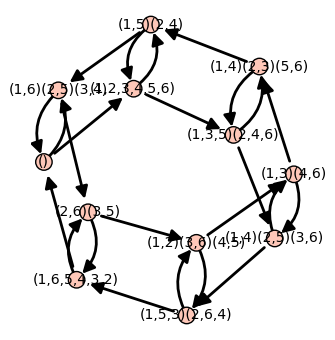
\includegraphics[width=0.7\textwidth]{caleygraph.png}
\end{columns}
\end{frame}


\begin{frame}[fragile]
\frametitle{Factoring}
\begin{description}
 \item[factor] uses {\tt Pari}
\begin{lstlisting}
sage: %time factor(next_prime(2^40) * next_prime(2^300))
CPU times: user 2.39 s, sys: 0.00 s, total: 2.39 s
Wall time: 2.41 s
1099511627791 * 203703597633448608626...
\end{lstlisting}

\item[ecm] uses {\tt GMP-ECM}

\begin{lstlisting}
sage: %time ecm.factor(next_prime(2^40) * next_prime(2^300))
CPU times: user 0.11 s, sys: 0.01 s, total: 0.12 s
Wall time: 0.82 s
[1099511627791, 203703597633448608626...
\end{lstlisting}

\item[qsieve] uses Bill Hart's {\tt qsieve} implementation
\begin{lstlisting}
sage: p, q = next_prime(2^90), next_prime(2^91)
sage: v,t = qsieve(p*q,time=True); t[:4]
2.26
\end{lstlisting}
\end{description}

\vspace{-1.2em}
\getinvolved{These should be unified to one command.}

\end{frame}

\begin{frame}[fragile,allowframebreaks]
\frametitle{Elliptic Curves}

\begin{columns}
\column{0.5\textwidth}
Sage is pretty good over $\mathbb{Q}$
\begin{lstlisting}
sage: E = EllipticCurve("37a")
sage: show(E.plot())
\end{lstlisting}
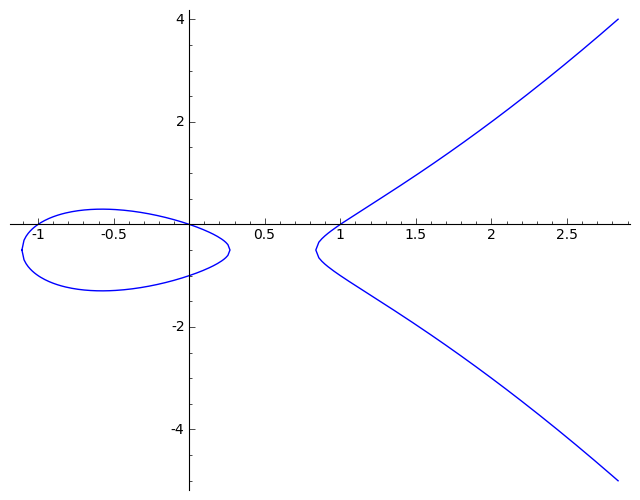
\includegraphics[width=1\textwidth]{elliptic_curve_over_q.png}
\column{0.5\textwidth}
\dots and okay over  $\mathbb{F}_p$
\begin{lstlisting}
sage: E = E.change_ring(GF(997))
sage: show(E.plot())
\end{lstlisting}
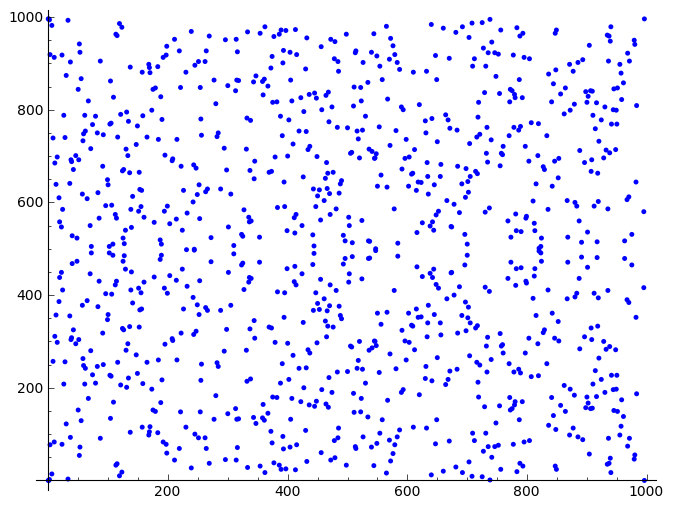
\includegraphics[width=1\textwidth]{elliptic_curve_mod_q.png}
\end{columns}

\framebreak

Basic operations over $\mathbb{F}_p$ are available

\begin{lstlisting}
sage: k = GF(next_prime(10^7))
sage: E = EllipticCurve(k, (k.random_element(),k.random_element()))
sage: E
Elliptic Curve defined by y^2 = x^3 + 7736620*x + 5470618
over Finite Field of size 10000019
sage: P = E.random_element()
sage: P.order()
499712
sage: 2*P + 1
(1070248 : 6510834 : 1)
\end{lstlisting}


\framebreak

Sage includes a fast implementation of the SEA (Schoff-Elkies-Atkin) algorithm for counting the number of points on an elliptic curve over $\F_p$.

\begin{lstlisting}
sage: K = GF(next_prime(10^20))
sage: E = EllipticCurve_from_j(k.random_element())
sage: E.cardinality()
99999999999371984255
\end{lstlisting}

Sage has the world's best code for computing $p$-adic regulators of elliptic curves. The $p$-adic regulator of an elliptic curve $E$ at a good ordinary prime $p$ is the determinant of the global $p$-adic height pairing matrix on the Mordell-Weil group $E(\mathbb{Q})$.

\begin{lstlisting}
sage: E = EllipticCurve('389a')
sage: E.padic_regulator(5, 10)
5^2 + 2*5^3 + 2*5^4 + 4*5^5 + 3*5^6 + 4*5^7 + 3*5^8 + 5^9 + O(5^11)
sage: E.padic_regulator(997, 10)
740*997^2 + 916*997^3 + 472*997^4 + 325*997^5 + 697*997^6
          + 642*997^7 + 68*997^8 + 860*997^9 + 884*997^10 + O(997^11)
\end{lstlisting}

\framebreak

Sage has the world's fastest implementation of computation of all integral points on an elliptic curve over $\mathbb{Q}$. This is also the only free open-source implementation available.

\vspace{1em}

(Apparently,) a very impressive example is the lowest conductor elliptic curve of rank $3$, which has 36 integral points.

\begin{lstlisting}
sage: E = elliptic_curves.rank(3)[0]
sage: E.integral_points(both_signs=True)   # less than 3 seconds
[(-3 : -1 : 1), (-3 : 0 : 1), ...(816 : -23310 : 1), (816 : 23309 : 1)]
\end{lstlisting}

\end{frame}

\begin{frame}[fragile,allowframebreaks]
\frametitle{Gröbner Bases}

\begin{lstlisting}
sage: K = GF(32003)
sage: T = TermOrder("deglex",2) + TermOrder("deglex",2)
sage: P.<w,x,y,z> = PolynomialRing(K,order=T)
sage: I = sage.rings.ideal.Katsura(P)
sage: [g.lm() for g in I.groebner_basis()] # Singular
[w, x, y*z^3, z^4, y^3, y^2*z]
sage: I.dimension()
0
sage: V = I.variety(); V
[{y: 0, z: 0, w: 1, x: 0}, {y: 0, z: 10668, w: 10668, x: 0}]
sage: J = I.change_ring(P.change_ring(QQ))
sage: J.variety()
[{y: 0, z: -32002/3, w: -32002/3, x: 0}, {y: 0, z: 0, w: -32002, x: 0}]
sage: len(J.variety(CC))
8
\end{lstlisting}

\framebreak

We estimate the complexity before solving:

\begin{lstlisting}
sage: n = 10; P = PolynomialRing(GF(32003), n, 'x')
sage: F = [P.random_element() for _ in range(P.ngens()+2)]
sage: s = random_vector(GF(32003),n)
sage: I = Ideal(f-f(*s) for f in F)
sage: D = I.degree_of_semi_regularity()
sage: D, log(binomial(n + D, n)^3, 2).n()
6, 34.65...
sage: I.groebner_basis('magma',prot='sage')
...
Leading term degree:  4. Critical pairs: 178.
Leading term degree:  5. Critical pairs: 515.
Leading term degree:  5. Critical pairs: 1155.
Leading term degree:  3. Critical pairs: 2845.
Leading term degree:  2. Critical pairs: 2850.
Leading term degree:  3. Critical pairs: 2795.
Leading term degree:  4. Critical pairs: 2605.
Leading term degree:  5. Critical pairs: 1609.
Leading term degree:  6. Critical pairs: 864 (all pairs ...
Leading term degree:  7. Critical pairs: 4 (all pairs ...
Leading term degree:  8. Critical pairs: 1 (all pairs ...

Highest degree reached during computation:  5.
[x0 + 7334, x1 - 12304, x2 - 7977, x3 - 8365, x4 - 7982, x5 + 676, ...]
\end{lstlisting}

\framebreak

Sage has a very good implementation of Gröbner basis computations over $\F_2[x_0,\dots,x_{n-1}]/\langle x_0^2 + x_0, \dots, x_{n-1}^2 + x_{n-1}\rangle$ thanks to {\tt PolyBoRi}.

\begin{lstlisting}
sage: B = BooleanPolynomialRing(50,'x',order='deglex')
sage: s = random_vector(GF(2),50)
sage: F = [B.random_element() for _ in range(500)]
sage: I = Ideal(f-f(*s) for f in F)
sage: G = I.groebner_basis(); G # PolyBoRi
Polynomial Sequence with 50 Polynomials in 50 Variables
sage: sorted(G)[0], s[0]
(x0 + 1, 1)
sage: I.variety()
[{x40: 0, x42: 1, x44: 0, ..., x23: 0, x25: 1}]
\end{lstlisting}

\end{frame}

\begin{frame}[fragile,allowframebreaks]
\frametitle{Mixed/Constraint Integer Programming}

Sage has a highlevel interface to Mixed Integer Linear solving

\begin{lstlisting}
sage: g = graphs.PetersenGraph()
sage: p = MixedIntegerLinearProgram(maximization=True)
sage: b = p.new_variable()
sage: p.set_objective(sum([b[v] for v in g]))
sage: for (u,v) in g.edges(labels=None):
...       p.add_constraint(b[u] + b[v], max=1)
sage: p.set_binary(b)
sage: p.solve(objective_only=True)
4.0
\end{lstlisting}


which supports many backends: {\tt GLPK}, {\tt Coin}, {\tt Gurobi}, {\tt CPLEX}.

\getinvolved{There is a patch bitrotting which adds a {\tt SCIP} interface to Sage. There's also some code which converts polynomial systems (with noise) to MIP/CIP awaiting integration into Sage.}

\end{frame}

\begin{frame}[fragile]
\frametitle{Graph Theory}
\begin{itemize}
\item builds on {\tt NetworkX} (Los Alamos's Python graph library)
\item graph isomorphism testing -- Robert Miller's new implementation
\item graph databases
\item 2d and 3d visualization
\end{itemize}
\begin{lstlisting}
sage: D = graphs.DodecahedralGraph()
sage: D.show3d()
\end{lstlisting}
\vspace{-5em}
\begin{flushright}
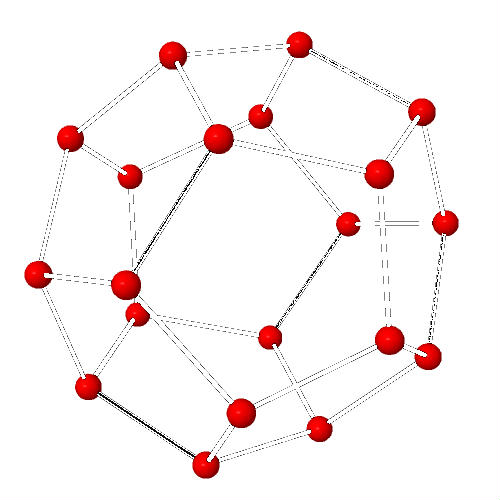
\includegraphics[width=0.3\textwidth]{graph3d.jpeg}
\end{flushright}
\vspace{-6em}
\begin{lstlisting}
sage: E = D.copy()
sage: gamma = SymmetricGroup(20).random_element()
sage: E.relabel(gamma)
sage: D.is_isomorphic(E)
True
sage: D.radius()
5
\end{lstlisting}
\end{frame}

\section{Cryptography}

\begin{frame}[fragile,allowframebreaks]
\frametitle{AES \& Equation Systems}

We construct small scale AES -- SR(1,1,1,4) -- over $\F_{2^4}$

\begin{lstlisting}
sage: sr = mq.SR(1,1,1,4); sr
SR(1,1,1,4)
sage: F,s = sr.polynomial_system() #zero inversions
...
<type 'exceptions.ZeroDivisionError'>: A zero inversion occurred ...

sage: F,s = sr.polynomial_system(); F # So we try again.
Polynomial System with 40 Polynomials in 20 Variables
\end{lstlisting}

\framebreak

We can export $F$ to {\tt Magma}:

\begin{lstlisting}
sage: magma(F)
Ideal of Polynomial ring of rank 20 over GF(2^4)
Graded Reverse Lexicographical Order
Variables: k100, k101, k102, k103, x100, x101, x102, x103, ...
Basis:
[
w100 + k000 + $.1^4,
w101 + k001 + $.1^8,
...
k000^2 + k001,
....
\end{lstlisting}

or to {\tt Singular}:

\begin{lstlisting}
sage: singular(F)
w100+k000+(a+1),
w101+k001+(a^2+1),
...
k002^2+k003,
...
\end{lstlisting}

\framebreak

Or we can use those systems transparently in the background:

\begin{lstlisting}
sage: F.groebner_basis() # Singular in the background
[k002 + (a^3 + 1)*k003 + (a^2),
 k001 + (a^3 + a^2)*k003 + (a^3),
 k000 + (a^2)*k003 + (a^3 + a^2),
 ...
\end{lstlisting}

\begin{lstlisting}
sage: F.groebner_basis(algorithm='magma') # Magma in the background
[k002 + (a^3 + 1)*k003 + (a^2),
 k001 + (a^3 + a^2)*k003 + (a^3),
 k000 + (a^2)*k003 + (a^3 + a^2),
 ...
\end{lstlisting}

\framebreak

Building blocks are also available individually:

\begin{lstlisting}
sage: sr.Lin
[   a^2 + 1     1   a^3 + a^2           a^2 + 1]
[         a     a           1 a^3 + a^2 + a + 1]
[   a^3 + a   a^2         a^2                 1]
[         1   a^3       a + 1             a + 1]

sage: sr = mq.SR(1, 1, 1, 8)
sage: R = sr.ring()
sage: xi = Matrix(R, 8, 1, sr.vars('x', 1))
sage: wi = Matrix(R, 8, 1, sr.vars('w', 1))
sage: sr.inversion_polynomials(xi, wi, 8)
[x100*w100 + 1, x101*w101 + 1, x102*w102 + 1, x103*w103 + 1,
 x104*w104 + 1, x105*w105 + 1, x106*w106 + 1, x107*w107 + 1]
\end{lstlisting}

\framebreak

Sage also provides AES equation systems over $\F_2$.

\begin{lstlisting}
sage: sr = mq.SR(2,1,1,4,gf2=True,polybori=True)
sage: F,s = sr.polynomial_system(); F
Polynomial System with 68 Polynomials in 36 Variables

sage: F.groebner_basis() # PolyBoRi
[k200 + k001 + k003 + 1,
 k201 + k001, k202 + 1,
 k203 + k000, x200 + k003,
 x201 + k000 + k001,
 x202 + k000 + k001 + k003,
 x203 + k000 + k003,
 w200 + k000 + k003 + 1,
 w201 + k001 + k003 + 1,
 w202 + k001 + 1,
 w203,
 ...
\end{lstlisting}

\framebreak

Interdependencies between polynomials:

\begin{lstlisting}
sage: sr = mq.SR(1,4,4,4,gf2=True,polybori=True, \
                         allow_zero_inversions=True)
sage: F,s = sr.polynomial_system()
sage: F_short = mq.MPolynomialSystem(F.ring(), F.rounds()[:-1])
sage: F_short.connected_components()
[Polynomial System with 80 Polynomials in 64 Variables,
 Polynomial System with 80 Polynomials in 64 Variables,
 Polynomial System with 80 Polynomials in 64 Variables,
 Polynomial System with 80 Polynomials in 64 Variables]

sage: S = mq.SBox(12,5,6,11,9,0,10,13,3,14,15,8,4,7,1,2)
sage: F_S = mq.MPolynomialSystem(S.polynomials(degree=3,groebner=True))
sage: F_S.connection_graph()
Graph on 8 vertices
\end{lstlisting}

\end{frame}

\begin{frame}[fragile,allowframebreaks]
\frametitle{S-Boxes}

Sage also supports some operations with S-boxes:

\begin{lstlisting}
sage: S = mq.SBox(12,5,6,11,9,0,10,13,3,14,15,8,4,7,1,2); S
(12, 5, 6, 11, 9, 0, 10, 13, 3, 14, 15, 8, 4, 7, 1, 2)
sage: type(S)
<class 'sage.crypto.mq.sbox.SBox'>
sage: S(0)
12
sage: S([0,0,0,1])
[0, 1, 0, 1]
sage: f = S.interpolation_polynomial()
sage: f(0), S(0)
(a^3 + a^2, 12)
\end{lstlisting}


\begin{eqnarray*}
f &=& a^{13}(x^{14} + x^{13}) + a^{6}(x^{12} + x^{6} + 1) + \\
 & &  a^{11}(x^{11} + x^4) + a^{14}(x^{10} + x^{9}) + \\
 & &  a^{10}(x^{8} + x^{3} + x^{2}) + a^{2}x^{7} + a^{9}x^{5}
\end{eqnarray*}

\framebreak

\begin{lstlisting}
sage: S = mq.SBox(12,5,6,11,9,0,10,13,3,14,15,8,4,7,1,2)
sage: S.linear_approximation_matrix()
[ 8  0  0  0  0  0  0  0  0  0  0  0  0  0  0  0]
[ 0  0  0  0  0 -4  0 -4  0  0  0  0  0 -4  0  4]
[ 0  0  2  2 -2 -2  0  0  2 -2  0  4  0  4 -2  2]
[ 0  0  2  2  2 -2 -4  0 -2  2 -4  0  0  0 -2 -2]
[ 0  0 -2  2 -2 -2  0  4 -2 -2  0 -4  0  0 -2  2]
[ 0  0 -2  2 -2  2  0  0  2  2 -4  0  4  0  2  2]
[ 0  0  0 -4  0  0 -4  0  0 -4  0  0  4  0  0  0]
[ 0  0  0  4  4  0  0  0  0 -4  0  0  0  0  4  0]
[ 0  0  2 -2  0  0 -2  2 -2  2  0  0 -2  2  4  4]
[ 0  4 -2 -2  0  0  2 -2 -2 -2 -4  0 -2  2  0  0]
[ 0  0  4  0  2  2  2 -2  0  0  0 -4  2  2 -2  2]
[ 0 -4  0  0 -2 -2  2 -2 -4  0  0  0  2  2  2 -2]
[ 0  0  0  0 -2 -2 -2 -2  4  0  0 -4 -2  2  2 -2]
[ 0  4  4  0 -2 -2  2  2  0  0  0  0  2 -2  2 -2]
[ 0  0  2  2 -4  4 -2 -2 -2 -2  0  0 -2 -2  0  0]
[ 0  4 -2  2  0  0 -2 -2 -2  2  4  0  2  2  0  0]
\end{lstlisting}

\framebreak

\begin{lstlisting}
sage: S = mq.SBox(12,5,6,11,9,0,10,13,3,14,15,8,4,7,1,2)
sage: S.difference_distribution_matrix()
[16  0  0  0  0  0  0  0  0  0  0  0  0  0  0  0]
[ 0  0  0  4  0  0  0  4  0  4  0  0  0  4  0  0]
[ 0  0  0  2  0  4  2  0  0  0  2  0  2  2  2  0]
[ 0  2  0  2  2  0  4  2  0  0  2  2  0  0  0  0]
[ 0  0  0  0  0  4  2  2  0  2  2  0  2  0  2  0]
[ 0  2  0  0  2  0  0  0  0  2  2  2  4  2  0  0]
[ 0  0  2  0  0  0  2  0  2  0  0  4  2  0  0  4]
[ 0  4  2  0  0  0  2  0  2  0  0  0  2  0  0  4]
[ 0  0  0  2  0  0  0  2  0  2  0  4  0  2  0  4]
[ 0  0  2  0  4  0  2  0  2  0  0  0  2  0  4  0]
[ 0  0  2  2  0  4  0  0  2  0  2  0  0  2  2  0]
[ 0  2  0  0  2  0  0  0  4  2  2  2  0  2  0  0]
[ 0  0  2  0  0  4  0  2  2  2  2  0  0  0  2  0]
[ 0  2  4  2  2  0  0  2  0  0  2  2  0  0  0  0]
[ 0  0  2  2  0  0  2  2  2  2  0  0  2  2  0  0]
[ 0  4  0  0  4  0  0  0  0  0  0  0  0  0  4  4]
\end{lstlisting}

\framebreak

\begin{lstlisting}
sage: S = mq.SBox(12,5,6,11,9,0,10,13,3,14,15,8,4,7,1,2)
sage: S.polynomials() #default: degree=2
[x1*x2 + x0 + x1 + x3 + y3,
 x0*x1 + x0*x2 + x0 + x1 + y0 + y2 + y3 + 1,
 x0*x3 + x1*x3 + x1*y0 + x0*y1 + x0*y2 + x1 + x2 + y2,
 x0*x3 + x0*y0 + x1*y1 + x0 + x2 + y2,
 x0*x2 + x0*y0 + x0*y1 + x1*y2 + x1 + x2 + x3 + y2 + y3, ...]
\end{lstlisting}

\begin{lstlisting}
sage: S = mq.SBox(12,5,6,11,9,0,10,13,3,14,15,8,4,7,1,2)
sage: P.<y0,y1,y2,y3,x0,x1,x2,x3> = PolynomialRing(GF(2),order='lex')
sage: X = [x0,x1,x2,x3]
sage: Y = [y0,y1,y2,y3]
sage: S.polynomials(X=X,Y=Y,degree=3,groebner=True)
[y0 + x0*x1*x3 + x0*x2*x3 + x0 + x1*x2*x3 + x1*x2 + x2 + x3 + 1,
 y1 + x0*x1*x3 + x0*x2*x3 + x0*x2 + x0*x3 + x0 + x1 + x2*x3 + 1,
 y2 + x0*x1*x3 + x0*x1 + x0*x2*x3 + x0*x2 + x0 + x1*x2*x3 + x2,
 y3 + x0 + x1*x2 + x1 + x3]
\end{lstlisting}
\end{frame}

\begin{frame}[fragile,allowframebreaks]
\frametitle{Boolean Functions}

\begin{lstlisting}
sage: from sage.crypto.boolean_function import *
sage: P.<x0,x1,x2,x3> = BooleanPolynomialRing()
sage: b = x0*x1 + x2*x3
sage: f = BooleanFunction(b)
sage: [b(x[0],x[1],x[2],x[3]) for x in GF(2)^4]
[0, 0, 0, 1, 0, 0, 0, 1, 0, 0, 0, 1, 1, 1, 1, 0]
sage: f.truth_table()
(False, False, False, True, False, False, False, True, False, False,
 False, True, True, True, True, False)
\end{lstlisting}

\framebreak

\begin{lstlisting}
sage: WT = f.walsh_hadamard_transform(); WT
(-4, -4, -4, 4, -4, -4, -4, 4, -4, -4, -4, 4, 4, 4, 4, -4)
sage: f.absolute_walsh_spectrum()
{4: 16}
sage: f.nonlinearity()
6
sage: 2^(4-1) - (1/2)*max([abs(x) for x in WT])
6
\end{lstlisting}

\framebreak

\begin{lstlisting}
sage: f.autocorrelation()
(16, 0, 0, 0, 0, 0, 0, 0, 0, 0, 0, 0, 0, 0, 0, 0)
sage: f.absolute_autocorrelation()
{16: 1, 0: 15}
sage: f.absolut_indicator() # this is a mis-spelling in Sage
0
sage: f.is_bent()
True
sage: f.is_balanced()
False
sage: f.is_symmetric()
False
sage: f.sum_of_square_indicator()
256
sage: f.correlation_immunity()
0
\end{lstlisting}

\begin{lstlisting}
sage: R.<x> = GF(2^8,'a')[]
sage: B = BooleanFunction(x^31)
sage: B.algebraic_immunity()
4
\end{lstlisting}
\end{frame}

\begin{frame}[fragile,allowframebreaks]
\frametitle{Lattice Generators}

Sage can generate many crypto-style lattices thanks to Richard Lindner and Michael Schneider.

\begin{itemize}
 \item Modular basis
\begin{lstlisting}
sage: sage.crypto.gen_lattice(m=10, seed=42)
[11  0  0  0  0  0  0  0  0  0]
[ 0 11  0  0  0  0  0  0  0  0]
[ 0  0 11  0  0  0  0  0  0  0]
[ 0  0  0 11  0  0  0  0  0  0]
[ 2  4  3  5  1  0  0  0  0  0]
[ 1 -5 -4  2  0  1  0  0  0  0]
[-4  3 -1  1  0  0  1  0  0  0]
[-2 -3 -4 -1  0  0  0  1  0  0]
[-5 -5  3  3  0  0  0  0  1  0]
[-4 -3  2 -5  0  0  0  0  0  1]
\end{lstlisting}
\framebreak
\item Random basis
\begin{lstlisting}
sage: sage.crypto.gen_lattice(type='random',n=1,m=10,q=11^4,seed=42)
[14641     0     0     0     0     0     0     0     0     0]
[  431     1     0     0     0     0     0     0     0     0]
[-4792     0     1     0     0     0     0     0     0     0]
[ 1015     0     0     1     0     0     0     0     0     0]
[-3086     0     0     0     1     0     0     0     0     0]
[-5378     0     0     0     0     1     0     0     0     0]
[ 4769     0     0     0     0     0     1     0     0     0]
[-1159     0     0     0     0     0     0     1     0     0]
[ 3082     0     0     0     0     0     0     0     1     0]
[-4580     0     0     0     0     0     0     0     0     1]
\end{lstlisting}
\framebreak
\item Ideal bases with quotient $x^n-1$, $m=2n$ are NTRU bases
\begin{lstlisting}
sage: sage.crypto.gen_lattice(type='ideal', seed=42, quotient=x^4-1)
[11  0  0  0  0  0  0  0]
[ 0 11  0  0  0  0  0  0]
[ 0  0 11  0  0  0  0  0]
[ 0  0  0 11  0  0  0  0]
[ 4 -2 -3 -3  1  0  0  0]
[-3  4 -2 -3  0  1  0  0]
[-3 -3  4 -2  0  0  1  0]
\end{lstlisting}
\framebreak
\item Cyclotomic bases with $n=2^k$ are SWIFFT bases
\begin{lstlisting}
sage: sage.crypto.gen_lattice(type='cyclotomic', seed=42)
[11  0  0  0  0  0  0  0]
[ 0 11  0  0  0  0  0  0]
[ 0  0 11  0  0  0  0  0]
[ 0  0  0 11  0  0  0  0]
[ 4 -2 -3 -3  1  0  0  0]
[ 3  4 -2 -3  0  1  0  0]
[ 3  3  4 -2  0  0  1  0]
[ 2  3  3  4  0  0  0  1]
\end{lstlisting}
\framebreak
\item Dual modular bases are related to Regev's famous public-key encryption
\begin{lstlisting}
sage: sage.crypto.gen_lattice(type='modular',m=10,seed=42,dual=True)
[ 0  0  0  0  0  0  0  0  0 11]
[ 0  0  0  0  0  0  0  0 11  0]
[ 0  0  0  0  0  0  0 11  0  0]
[ 0  0  0  0  0  0 11  0  0  0]
[ 0  0  0  0  0 11  0  0  0  0]
[ 0  0  0  0 11  0  0  0  0  0]
[ 0  0  0  1 -5 -2 -1  1 -3  5]
[ 0  0  1  0 -3  4  1  4 -3 -2]
[ 0  1  0  0 -4  5 -3  3  5  3]
[ 1  0  0  0 -2 -1  4  2  5  4]
\end{lstlisting}
\end{itemize}

\end{frame}

\section{External Tools, Ciphers}

\begin{frame}[allowframebreaks,fragile]
\frametitle{DES}

An equation system generator for DES is available at \url{http://bitbucket.org/malb/algebraic_attacks}.

\begin{lstlisting}
sage: attach des.py
sage: des = DES(Nr=2,sbox_eq='cubic') #sopns, sopns_gb
sage: F,s = des.polynomial_system()
Pre-computing fully cubic S-Box equations.
sage: F
Polynomial System with 1856 Polynomials in 120 Variables
sage: F_easy = F.subs(s); F_easy
Polynomial System with 1856 Polynomials in 64 Variables
sage: %time gb = F_easy.groebner_basis()
CPU times: user 0.20 s, sys: 0.01 s, total: 0.22 s
Wall time: 0.32 s
sage: gb[:5]
[y0100, y0101, y0102, y0103 + 1, y0104]

sage: %time gb = F.groebner_basis()
CPU times: user 0.42 s, sys: 0.00 s, total: 0.42 s
Wall time: 0.47 s
sage: gb[:5]
[k00 + 1, k01, k02, k03 + 1, k04 + 1]
\end{lstlisting}

\framebreak

S-boxes are available independently:

\begin{lstlisting}
sage: S1 = DESSBox(1)
sage: S1.polynomials(degree=3)
... # a long long list
sage: print S1.difference_distribution_matrix().str()
[64  0  0  0  0  0  0  0  0  0  0  0  0  0  0  0]
[ 0  0  0  6  0  2  4  4  0 10 12  4 10  6  2  4]
[ 0  0  0  8  0  4  4  4  0  6  8  6 12  6  4  2]
[14  4  2  2 10  6  4  2  6  4  4  0  2  2  2  0]
[ 0  0  0  6  0 10 10  6  0  4  6  4  2  8  6  2]
[ 4  8  6  2  2  4  4  2  0  4  4  0 12  2  4  6]
[ 0  4  2  4  8  2  6  2  8  4  4  2  4  2  0 12]
[ 2  4 10  4  0  4  8  4  2  4  8  2  2  2  4  4]
[ 0  0  0 12  0  8  8  4  0  6  2  8  8  2  2  4]
[10  2  4  0  2  4  6  0  2  2  8  0 10  0  2 12]
[ 0  8  6  2  2  8  6  0  6  4  6  0  4  0  2 10]
[ 2  4  0 10  2  2  4  0  2  6  2  6  6  4  2 12]
[ 0  0  0  8  0  6  6  0  0  6  6  4  6  6 14  2]
...
\end{lstlisting}
\end{frame}

\begin{frame}[fragile]
\frametitle{PRESENT}

An equation system generator for PRESENT is also available.

\begin{lstlisting}
sage: attach present.py
sage: p = PRESENT(Nr=1)
sage: F,s = p.polynomial_system(); F
Polynomial System with 502 Polynomials in 212 Variables
sage: R = F.ring()
sage: R.gens()[:16]
(K0000, K0001, K0002, K0003, K0004, K0005, K0006, ...)
sage: K_guess = R.gens()[:16] # 80 - 64 = 16
sage: guess = dict([(k,GF(2).random_element()) for k in K_guess])
sage: F_guessed = F.subs(guess); F_guessed
Polynomial System with 502 Polynomials in 196 Variables
sage: F_target = F_guessed.eliminate_linear_variables()
sage: F_target
Polynomial System with 260 Polynomials in 42 Variables
sage: F_target.groebner_basis()
[1]

sage: guess = dict([(k,s[k]) for k in K_guess])
sage: F_guessed = F.subs(guess)
sage: F_target = F_guessed.eliminate_linear_variables();
sage: gb = F_target.groebner_basis()
sage: gb[-1]
K0070
\end{lstlisting}
\end{frame}

\section{Example Application}

\begin{frame}[fragile]
\frametitle{LWE in 10 lines}
\begin{lstlisting}
sage: n = 10
sage: q = random_prime(n^2,2*n^2); K = GF(q)
sage: VS = VectorSpace(K,n)
sage: s = VS.random_element()
sage: chi = lambda: K(round(gauss(0,sqrt(n))))
sage: def sample():
....:     a = VS.random_element()
....:     return a, a.dot_product(s)+chi()
....:
sage: sample()
((3, 7, 7, 0, 12, 6, 13, 15, 15, 10), 5)
\end{lstlisting}

\begin{thebibliography}{ff}
\bibitem{lwesurvey}
O.\ Regev.
\newblock The learning with errors problem.
\newblock In {\em IEEE Conf.\ on Comp.\ Complexity 2010}, pages
  191--204, 2010.
\end{thebibliography}


\end{frame}

\begin{frame}[fragile,allowframebreaks]
\frametitle{Homomorphic Encryption}

First, \textbf{KeyGen}:

\begin{lstlisting}
ZZrand = lambda x,y: ZZ.random_element(x,y)

class IHE:
  def __init__(self, l):
    self.rho, self.rhoprime, self.eta = l, 2*l, l**2
    self.gamma, self.tau = l**5, l**5 + l

    p = ZZrand(2**(self.eta-1),2**self.eta)
    self.p = p if p%2 != 0 else p+1

    while True:
        x = []
        for i in xrange(self.tau+1):
            x.append( self.sample() )
        x.sort(reverse=True)
        if x[0]%2 == 1 and IHE.mod(x[0],p)%2 == 0:
            break
    self.x = x
\end{lstlisting}

\framebreak

Now, \textbf{Sample}, \textbf{Encrypt} and \textbf{Decrypt}:

\begin{lstlisting}
  def sample(self):
    q = ZZrand(0, ceil(2**self.gamma/self.p))
    r = ZZrand(-(2**self.rho) + 1, 2**self.rho)
    return q*self.p + r

  @staticmethod
  def mod(x,p):
    x = x % p #Sage normalises between [0,p), but we need (-p/2,p/2]
    return x - p if x > p//2 else x

  def encrypt(self, m):
    S = range(1,self.tau+1)
    shuffle(S)
    S = S[:ceil(log(self.rho))]
    r = ZZrand(-(2**self.rhoprime)+1,2**self.rhoprime)
    c = m%2 + 2*r + 2*sum(self.x[i] for i in S)
    return IHE.mod(c, self.x[0])

  def decrypt(self, c):
    return IHE.mod(c, self.p)%2
\end{lstlisting}


\framebreak

Let's try it:

\begin{lstlisting}
sage: attach integer_homomorphic_short.py
sage: ihe = IHE(5)
sage: ihe.decrypt(ihe.encrypt(0) + ihe.encrypt(1))
1
sage: ihe.decrypt(ihe.encrypt(0) * ihe.encrypt(1))
0
sage: ihe.decrypt(ihe.encrypt(1) * ihe.encrypt(1))
1
\end{lstlisting}

\begin{flushright}
\dots somewhat homomorphic encryption in 29 lines of code.
\end{flushright}

\begin{thebibliography}{FOO}
\bibitem{DGHV10}
M.\ van Dijk, C.\ Gentry, S.\ Halevi, and V.\ Vaikuntanathan.
\newblock Fully homomorphic encryption over the integers.
\newblock In {\em EUROCRYPT 2010}, volume 6110 of {\em LNCS}, pages 24--43, 2010.
\end{thebibliography}

\end{frame}

\begin{frame}[fragile]
\frametitle{ElimLin}

\begin{lstlisting}
sage: P.<x1,x2,x3,x4,x5> = BooleanPolynomialRing()
sage: f1 = x1*x2 + x1*x3 + x2*x5 + x3*x5 + x2 + x4 + x5 + 1
sage: f2 = x1*x3 + x1*x4 + x2*x3 + x2*x4
sage: f3 = x1*x4 + x2*x3 + x3 + 1
sage: f4 = x1*x4 + x1*x5 + x2*x5 + x1
sage: f5 = x1*x5 + x2*x3 + x3*x5 + x1 + x3 + x4
sage: f6 = x1*x5 + x2*x3 + x3*x5 + x5 + x4 + x2 + 1
sage: I = Ideal(f1,f2,f3,f4,f5,f6)
sage: S,R = I.gens(),list()
sage: while max(f.degree() for f in S) > 1:
...      S = Sequence(sage.rings.polynomial.pbori.gauss_on_polys(S))
...      S,r = S.eliminate_linear_variables(100,lambda a,b:False,True)
...      R.extend(r)
sage: R.extend(S)
sage: Sequence(sage.rings.polynomial.pbori.gauss_on_polys(R))
[x1, x2, x3 + 1, x4 + 1, x5]
sage: I.interreduced_basis() # "ElimLin"
[x1, x2, x3 + 1, x4 + 1, x5]
\end{lstlisting}

\begin{thebibliography}{FOOBAR}
\bibitem{CSSV12}
  N.\ Courtois, P.\ Sepehrdad, P.\ Susil and S.\ Vaudenay.
  \newblock ElimLin Algorithm Revisited.
  \newblock in {\em FSE 2012}. Springer Verlag, 2012.
\end{thebibliography}


\end{frame}


\end{document}
